\documentclass[11pt,a4paper]{article}
\usepackage{graphicx}
\usepackage{titling}
\usepackage{pdfpages}
\usepackage{tikz}
\usetikzlibrary{shapes}
\usepackage{amssymb}
\usepackage{forest}
\begin{document}
\author{Ankur Dhoot}
\title{CS 471 HW 2}
\maketitle


\section*{Q1}

\paragraph*{(a)}
\begin{center}
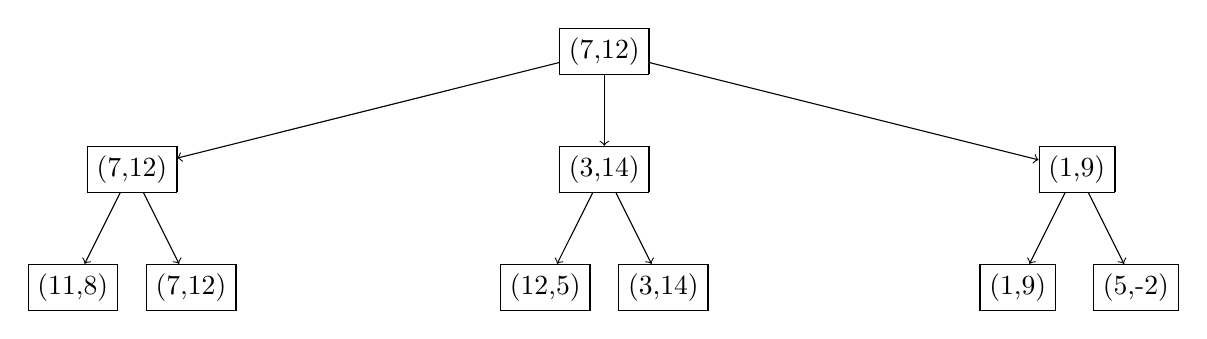
\begin{tikzpicture}
\tikzstyle{bplus}=[rectangle split, rectangle split horizontal,rectangle split ignore empty parts,draw]
\tikzstyle{every node}=[bplus]
\tikzstyle{level 1}=[sibling distance=60mm]
\tikzstyle{level 2}=[sibling distance=15mm]
\node {(7,12)} [->]
  child {node {(7,12)}
    child {node {(11,8)}}
    child {node {(7,12)}}   
  } 
  child {node {(3,14)}
    child {node {(12,5)}}
    child {node {(3,14)}}   
  } 
  child {node {(1,9)}
    child {node {(1,9)}}
    child {node {(5,-2)}}   
  } 
;\end{tikzpicture}
\end{center}

\paragraph*{(b)}
Suppose we're at a node corresponding to Player B. We have values $\alpha$ and $\beta$ corresponding to the value of the best choice for Player A and Player B, respectively, that we have found so far. We are given that $|U_{A}$ + $U_{B}|$ $\leq k$. Suppose we explore from the current node and find that $U_{B} \geq k - \alpha$. This implies $U_{A} \leq \alpha$ by our given constraint. Thus, we don't need to further explore paths from the current node and the node can be pruned. The analogous inequalities hold if we're at a node corresponding to Player A.

\section*{Q2}
\paragraph*{(a)}
A possible fitness function would be defined by counting the number of digits (starting at the third digit) in the sequence that are equal to the sum of the previous two and dividing by the length of the sequence (after the first two digits). So the sequence 1 2 3 4 would have fitness score 1/2. Essentially, it the fitness function gives the fraction of "correct" digits in the sequence. If the sequence is shorter than 3, trivially define the fitness function to return 1.

\paragraph*{(b)}
If the sequences are fixed length, it's possible that making local changes to the sequence (i.e changing any one digit in the sequence) will not improve the fitness function. We might make a given position in the sequence the sum of the previous two, but this could break the rule on one of the next two digits. For example, the sequence 1 4 5 8 cannot be improved (according to the score function) by changing a single digit. Thus, we could get stuck on plateaus or local minima. 

\paragraph*{(c)}
If we permit sequences to be of arbitrary length (i.e we can add or remove a digit in our local search), we are guaranteed to not get stuck in plateaus or local minima. The reason is that we can always add a digit at the end of the sequence that is the sum of the previous two, and this can only increase the score of our fitness function (e.g if our current sequence scores (2/5) the new sequence will score (3/6) which is strictly greater always). Or if the last digit isn't a sum of the previous two, we can just delete it (e.g if our current sequence scores (2/5) our new sequence scores (2/4) which is strictly greater). Thus, there is always a decision that local search can make that increases the fitness score.

\section*{Q3}

We're given the following:

$A \wedge B \Rightarrow D$

$Q \wedge \neg R \Rightarrow A$

$\neg Q \vee \neg B \vee \neg R$

$P \Rightarrow Q$

$P \Rightarrow B$

$B \Rightarrow P$

$B$
\paragraph*{(a)}

We'll prove $D$ using forward chaining where we check to see if premises are satisfied and if so, add the conclusion to our inferred set:

First note that we'll rewrite $\neg Q \vee \neg B \vee \neg R$ as $Q \wedge B \Rightarrow \neg R$. 

$B$  \qquad (B is inferred)
 
$B \Rightarrow P$   \qquad (B and P are inferred)

$P \Rightarrow Q$   \qquad(B, P, Q are inferred) 

$Q \wedge B \Rightarrow \neg R$  \qquad (B, P, Q, $\neg R$ are inferred)

$Q \wedge \neg R \Rightarrow A$  \qquad (B, P, Q, $\neg R$, A are inferred)

$A \wedge B \Rightarrow D$     \qquad (B, P, Q, $\neg R$, A, D are inferred)

\paragraph*{(b)}

Using backward chaining we'll identify the premises we must satisfy recursively:

$D$

$A \wedge B \Rightarrow D$

$Q \wedge \neg R \Rightarrow A$

$P \Rightarrow Q$

$B \Rightarrow P$

$B$

$Q \wedge B \Rightarrow \neg R$


In search tree form, read left to right as in DFS (similar to Figure 9.7 in RN):
\begin{center}
\begin{tikzpicture}
\tikzstyle{bplus}=[rectangle split, rectangle split horizontal,rectangle split ignore empty parts,draw]
\tikzstyle{every node}=[bplus]
\tikzstyle{level 1}=[sibling distance=60mm]
\tikzstyle{level 2}=[sibling distance=15mm]
\node {D} [->]
  child {node {A}
    child {node {Q}
    	child {node {P}
    		child {node {B}}
    	}
    }
    child {node {$\neg$R}
    	child {node {Q}}
    	child {node {B}}
    }   
  } 
  child {node {B}
  }  
;\end{tikzpicture}
\end{center}

\section*{Q4}
\paragraph*{(a)}

1. Captain(Enterprise, Kirk)

2. $\exists x$ $\forall y$ HasDisease(y,x) $\Rightarrow$ Hungry(y)

3. $\forall x$ OnShip(Enterprise, x) $\Rightarrow$ $\neg$ Diseased(x)

4. Pizzas(Kirk)

5. $\forall x$ Pizzas(x) $\Rightarrow$ Hungry(x)

6. $\forall x$ [$\exists y$ Captain(y, x)] $\Rightarrow$ OnShip(x, y)

7. Hungry(Kirk) $\Leftrightarrow$ Sick(Kirk)

\paragraph*{(b)}

1. Captain(Enterprise, Kirk)

2. $\neg$ HasDisease(y, C1) $\vee$ Hungry(y)     (Skolem Constant C1)

3. $\neg$ OnShip(Enterprise, x) $\vee$ $\neg$ Diseased(x)

4. Pizzas(Kirk)

5. $\neg$ Pizzas(x) $\vee$ Hungry(x)

6. $\forall x$ $\neg$[$\exists y$ Captain(y, x)] $\vee$ OnShip(x, y)

$\forall x$ [$\forall y$ $\neg$ Captain(y, x)] $\vee$ OnShip(x, y)  \qquad(using rules for negated quantifiers)

$\neg$ Captain(y, x) $\vee$ OnShip(x, y)        \qquad(after removing universal quantifiers)

7. ($\neg$ Hungry(Kirk) $\vee$ Sick(Kirk)) $\wedge$ ($\neg$ Sick(Kirk) $\vee$ Hungry(Kirk))

\paragraph*{(c)}
We'll add a couple common sense sentences:
$\forall x$ Sick(x) $\Rightarrow$ Diseased(x)

which converts to $\neg$ Sick(x) $\vee$ Diseased(x)

1. Pizzas(Kirk)

$\neg$ Pizzas(x) $\vee$ Hungry(x)

$\therefore$ Hungry(Kirk)
\newline

2. Hungry(Kirk)

$\neg$ Hungry(Kirk) $\vee$ Sick(Kirk)

$\therefore$ Sick(Kirk)
\newline

3. Sick(Kirk)

$\neg$ Sick(x) $\vee$ Diseased(x)

$\therefore$ Diseased(Kirk)
\newline

4. Diseased(Kirk)

$\neg$ OnShip(Enterprise, x) $\vee$ $\neg$ Diseased(x)

$\therefore$ $\neg$ OnShip(Enterprise, Kirk)
\newline

5. $\neg$ OnShip(Enterprise, Kirk)

$\neg$ Captain(y, x) $\vee$ OnShip(x, y) 

$\therefore$ $\neg$ Captain(Enterprise, Kirk)

so we've reached a contradiction.

In words: Kirk ate several whole pizzas for lunch meaning he was hungry. Kirk is only hungry when he is sick. Thus, Kirk is sick, which also means Kirk is diseased. Since the Enterprise doesn't have any diseases, Kirk is not on the Enterprise. Since the caption of a ship must remain on a ship, Kirk cannot be the captain of the Enterprise, a contradiction.

\section*{Q5}

\paragraph*{(a)}

\begin{center}
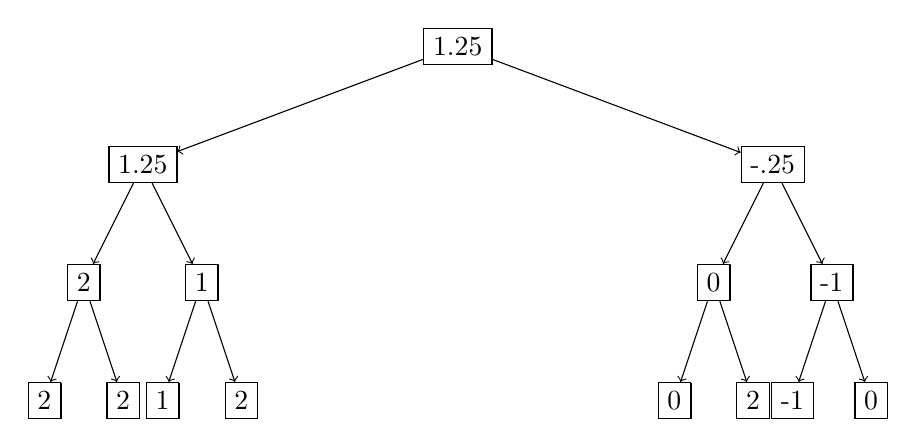
\begin{tikzpicture}
\tikzstyle{bplus}=[rectangle split, rectangle split horizontal,rectangle split ignore empty parts,draw]
\tikzstyle{every node}=[bplus]
\tikzstyle{level 1}=[sibling distance=80mm]
\tikzstyle{level 2}=[sibling distance=15mm]
\tikzstyle{level 3}=[sibling distance=10mm]
\node {1.25} [->]
  child {node {1.25}
    child {node {2}
    	child {node {2}}
    	child {node {2}}
    }
    child {node {1}
    	child {node {1}}
    	child {node {2}}
    }   
  } 
  child {node {-.25}
  	child {node {0}
  		child {node {0}}
  		child {node {2}}
  	}
  	child {node {-1}
  		child {node {-1}}
  		child {node {0}}
  	}
  }  
;\end{tikzpicture}
\end{center}

The optimal decision at the root is to go left.

\paragraph*{(b)}
Yes, we do need to evaluate the seventh and eighth leaves. Those two leaves have no constraint on them, and could thus take any possible value. For example, if both nodes have value $>$ 5, then the min node immediately above will have value $>$ 5 so that the chance node on the right will have value $>$ 1.25 meaning the optimal decision at the root will change from left to right.

\paragraph*{(c)}
We only need to evaluate the first five leaves. We already know that we can attain an expected max value of 1.25 at the root after evaluating the first four leaves. When we evaluate the fifth leaf, and see it has value 0, then we know the min node above it has to be at most 0. We need to show that the optimal decision at the root now remains to go left regardless of the value at the other three leaves. 

Thus it suffices to suppose that the other three leaves take on the max value of 2. Then the left min node will take on value 0 and the right min node value 2. This means the chance node will take on value .75 * 0 + .25 * 2 = .5. But the max node can already attain an expected value of 1.25 by going left, so the optimal decision for the max node remains to go left. 

Thus only the first five leaves need be evaluated.

\paragraph*{(d)}
We need to show that the decisions at each level of the search tree are the same.

Let T denote the original search tree and T' denote the tree after scaling the leaf values. We'll show that at every node n' in T' corresponding to n in T, the value of that node v(n') = av(n) + b.

We'll refer to depth in this proof as the distance from the bottom of the tree (the leaves). 

Base Case: Clearly true for the leaves since we applied the linear transform to each leaf value.

Now suppose it's true for all nodes up till depth d. We must show it's true for depth d+1.

If the nodes at depth d+1 are chance nodes:

Let $\alpha$ denote the set of actions from a given chance node, n', in state s. Let U'(s,a) denote the expectimax value of taking action r from state s in tree T'. 

$$v(n') = \sum_{r \in \alpha} P(r)U'(s,r) = \sum_{r \in \alpha} P(r)(aU(s,r) + b)$$

$$ = a \sum_{r \in \alpha} P(r)U(s,r) + b\sum_{r \in \alpha} P(r) = a \sum_{r \in \alpha} P(r)U(s,r) + b = av(n) + b$$

where the second equality follows by the induction hypothesis. 
\newline

If the nodes at depth d+1 are max nodes:

Expectimax will select the child with the highest expectimax value. Suppose in tree T, this was child $c_{*}$. That means the node took on value v($c_{*}$) in T and v($c_{*}$) $>$ v($c_{i}$) for any child $c_{i} \neq c_{*}$.  By the induction hypothesis, v($c_{*}^{'}$) = av($c_{*}$) + b $>$ av($c_{i}$) + b = v($c_{i}^{'}$) for any child $c_{i}^{'} \neq c_{*}^{'}$. Thus, the max node will take on value v($c_{*}^{'}$) = av($c_{*}$) + b and will thus make the same decision in T' as in T.
\newline

If the nodes at depth d+1 are min nodes:

Use an analagous proof to above except taking the minimum over all children. 

Thus, by induction, we've shown under a positive linear transformation, expectimax search decisions remain the same.



\end{document}